% !TeX spellcheck = en_US
\documentclass[letterpaper,12pt,twoside]{report}
\usepackage{fancyhdr}
\usepackage{fullpage}
\usepackage{tikz}
\usepackage{amsmath}
\usepackage{textcomp}
\usepackage{graphicx}
\usepackage{calc}

\begin{document}
	\pagestyle{fancy}
	\fancyhf{}
	\fancyhead[L]{Day 23}
	\fancyhead[R]{\textit{The Calendar Project}}
	\fancyfoot[L]{Citations Involved: none}
	
	% Problem
	\paragraph{Problem}
	\begin{quote}
		\textsf{Diagonal $AC$ in square $ABCD$ is a
			chord of a circle with radius 12 cm. If $\textrm{m}\widehat{AC} = 30$\textdegree, what is the area of $ABCD$?}
	\end{quote}
	
	% Graphics
	\begin{center}
		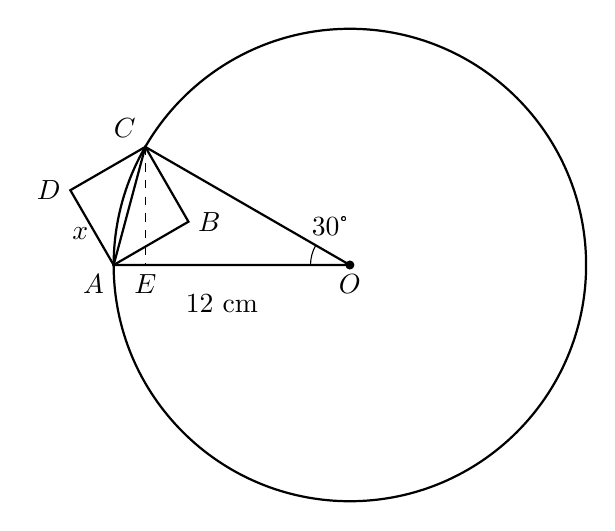
\begin{tikzpicture}[scale=0.25]
		\draw[thick] (0,0) circle [radius=12];
		\draw[fill=black] (0,0) circle [radius=0.2];
		\node[below] at (0,0) {$O$};
		
		\draw[thick] (0,0) -- (-12,0) -- (-10.3923,6) -- cycle;
		\node[below left] at (-12,0) {$A$};
		\node[above left] at (-10.3923,6) {$C$};
		\node[below] at (-6.5,-1) {12 cm};
		\draw (-2,0) arc [radius=2,start angle=180, end angle=150];
		\node[above] at (-1,1) {30\textdegree};
		
		\draw[thick] (-10.3923,6) -- (-8.2,2.2) -- (-12,0) -- (-14.2,3.8) -- cycle;
		\node[right] at (-8.2,2.2) {$B$};
		\node[left] at (-14.2,3.8) {$D$};
		\node[left] at (-12.8,1.6) {$x$};
		
		\draw[dashed] (-10.3923,6) -- (-10.3923,0);
		\node[below] at (-10.3923,0) {$E$};
		
		\end{tikzpicture}
	\end{center}
	
	% Reasoning
	\paragraph{Reasoning}
	\begin{quotation}
		
		As shown above, the center of the circle is denoted as $O$.
		
		Draw $\overline{CE}$ such that it is perpendicular to $\overline{AO}$, which makes $\angle CEO$ and $\angle CEA$ right angles by definition. This makes $\triangle CEO$ and $\triangle CEA$ right triangles. Since $\angle CEO$ is a right angle, it has a measure of 90\textdegree. With a 90\textdegree   \space angle and a 30\textdegree \space angle ($\angle EOC$), m$\angle OCE$ can be determined by the Triangle Sum Theorem: $\text{m}\angle CEO+\text{m}\angle EOC+\text{m}\angle OCE=180\text{\textdegree} \Rightarrow 90+30+\text{m}\angle OCE=180 \Rightarrow 120+\text{m}\angle OCE=180 \Rightarrow \text{m}\angle OCE=180-120 \Rightarrow \text{m}\angle OCE=60$\textdegree. Thus, $\triangle CEO$ can be classified as a 30\textdegree-60\textdegree-90\textdegree \space triangle. $\overline{CO}$, its hypotenuse, is a radius of circle O; $\overline{AO}$ is also a radius of circle O. Since all radii are congruent, $\overline{AO}\cong\overline{CO}$; given that circle $O$'s radius is 12, $CO=AO=12$. By the 30\textdegree-60\textdegree-90\textdegree \space Triangle Theorem, $CE=\frac{1}{2}CO$ and $EO=CE\sqrt{3}$. By substitution, $CE=\frac{1}{2}(12)=6$ and $EO=6\sqrt{3}$.
		
		By the SAP, $AE+EO=AO$. By substitution, $AE+6\sqrt{3}=12$; when $6\sqrt{3}$ is subtracted from both sides, $AE=12-6\sqrt{3}\approx 1.6$. Since $\triangle AEC$ is a right triangle, the Pythagorean Theorem can be applied: $a^2+b^2=c^2 \Rightarrow AE^2+CE^2=AC^2 \Rightarrow (12-6\sqrt{3})^2+6^2=AC^2 \Rightarrow (144-144\sqrt{3}+108)+36=AC^2 \Rightarrow 288-144\sqrt{3}=AC^2$.
		
		Since a square is also a rhombus, the rhombus area formula ($\frac{1}{2}d_1 d_2$ where $d_1$ and $d_2$ are its diagonals) is applicable to square $ABCD$. A rectangle's diagonals are congruent; since a square is also a rectangle, square $ABCD$'s diagonals are congruent. As such, $AC=BD$ and the square's area is $\frac{1}{2}d_1 d_2=\frac{1}{2}(AC)(BD)=\frac{1}{2}(AC)(AC)=\frac{1}{2}AC^2=\frac{1}{2}(288-144\sqrt{3})=\boxed{144-72\sqrt{3}\text{  cm}^2}$.
			
\end{quotation}
	
	
\end{document}